% TODO: GENERAL CHECKUP NEEDED

\section{Poison Kin}
\begin{linenumbers}
\DndDropCapLine{T}{hey're a poison spilled down onto}
\textit{ our world, I tell ya'!
Grungs're bad.
They real bad!
They tell ya' their skin be the worst part o'em, but they don't know!
The spears mon.
It's the spears!}

\hspace*{\fill} --- Kleeck recounts her brief visit to Mabela.

Also known as grungs, the poison kin are aggressive creatures that look similar to dart frogs.
The species quickly settled into the chirping wilds and the areas surrounding the rainforest after their arrival during the schism.
They are fiercely territorial and see themselves as superior to most other creatures.

\subsection*{Class Structure}
Grung society is a caste system.
Each caste lays eggs in a separate hatching pool, and juvenile grungs join their caste upon emergence from their hatchery.
All grungs are a dull greenish gray when they are born, but each individual takes on the color of its caste as it grows to adulthood.
From lowest to highest caste, grungs are green, blue, purple, red, orange, and gold.

Green grungs are the tribe's warriors, hunters, and laborers, and blue grungs work as artisans and in other domestic roles.
Supervising and guiding both groups are the purple grungs, which serve as administrators and commanders.
Red grungs are the tribe's scholars and sorcerers.
They are superior to purple, blue, and green grungs and given proper respect even by the grungs of higher status.
Higher castes include orange grungs, which are elite warriors that have authority over all lesser grungs, and gold grungs, which hold the highest leadership positions.
A tribe's sovereign is always a gold grung.

A grung normally remains in its caste for life.
On rare occasions, an individual that distinguishes itself with great deeds can earn an invitation to join a higher caste.
A mixture of godsblood, seawater and poison is blessed by a red grung, and by drinking it the elevated grung changes color and is inducted into its new caste in the same way that a juvenile of the caste would be.
From then on, the grung and its progeny are members of the higher caste.

\subsection*{Poisonous Skin}
All grungs secrete a substance that is harmless to them but poisonous to other creatures.
A grung can also use this secretion as venom to coat its weapons.
Grungs are always on the lookout for creatures they can capture and enslave, and use slaves for all manner of menial tasks and hard labor.
Slaves are fed mildly poisoned food to keep them lethargic and compliant.
A creature afflicted in this way over a long period of time becomes a shell of its former self, and it seldom can be restored to normalcy.
Being amphibious, grungs require water to live; any grung that fails to immerse itself in water for at least 1 hour during a day becomes quite exhausted.

\subsection*{Whistle Stick}
All grungs are trained to use a musical instrument called the whistle-stick.
This is a hollow wooden tube with holes cut throughout, much like a flute.
Grungs play music with it for entertainment, but can also swing it about by a sturdy cord to create a sound recognizable by others of their kin, so they know each other's approximate location.
Additionally, any creature that can speak the krehlo language can use a whistle stick in this manner to communicate over distance.

\subsection*{Outcast or Voyager}
Since social advancement among grungs can only be achieved by a great deed, it is not unusual for a grung or a small group of them to travel around the coasts and rivers of Yuadrem.
They attempt to obtain renown by murdering an enemy of their civilization, or by bringing a rare artifact or important strategic information.

While a rare occurrence, sometimes an individual grung or even entire family-lines can grow disillusioned by the hardships of class advancements.
Some of them decide to escape from their cities, leading lives of their own as independent colonies or as members of the rare cities or towns willing to accept them.
Individuals from these groups are known to follow a life of adventure to help their communities or simply to satiate an internal need for excitement in the grung's heart.

\subsection*{Grung Names}
Grungs usually have simple, non-gender-specific names with a strong consonant joined by a syllable with a glottal stop, but members of higher castes prefer longer, more elaborate names to reflect their status.
Their names don't actually come from the krelho language, but are made based on what's easier to pronounce for the grung.
Grungs also wear their city of origin as surname.

\paragraph{Names}
B'ang, B'leep, B'lip, B'loop, Bl'eg, Bl'myeek, Bl'ngiip, Ch'eg, Ch'rol, D'aht, D'khan, F'huu, Fl'aak, Fl'uup, G'lahp, Gh'rol, K'eet, K'riig, K'ung, R'ang, R'loo.

\paragraph{Surnames} Bakagar, Bomqueeg, Gor, Int, Joppank, Kangaru, Limlim, Mabela, Obu, Om, Ploqlek, Queequio, Quott'nem, Uhok'moa, Wewat, Xilkoko, Zipqueg.

\begin{figure}[!t]
    \centering
    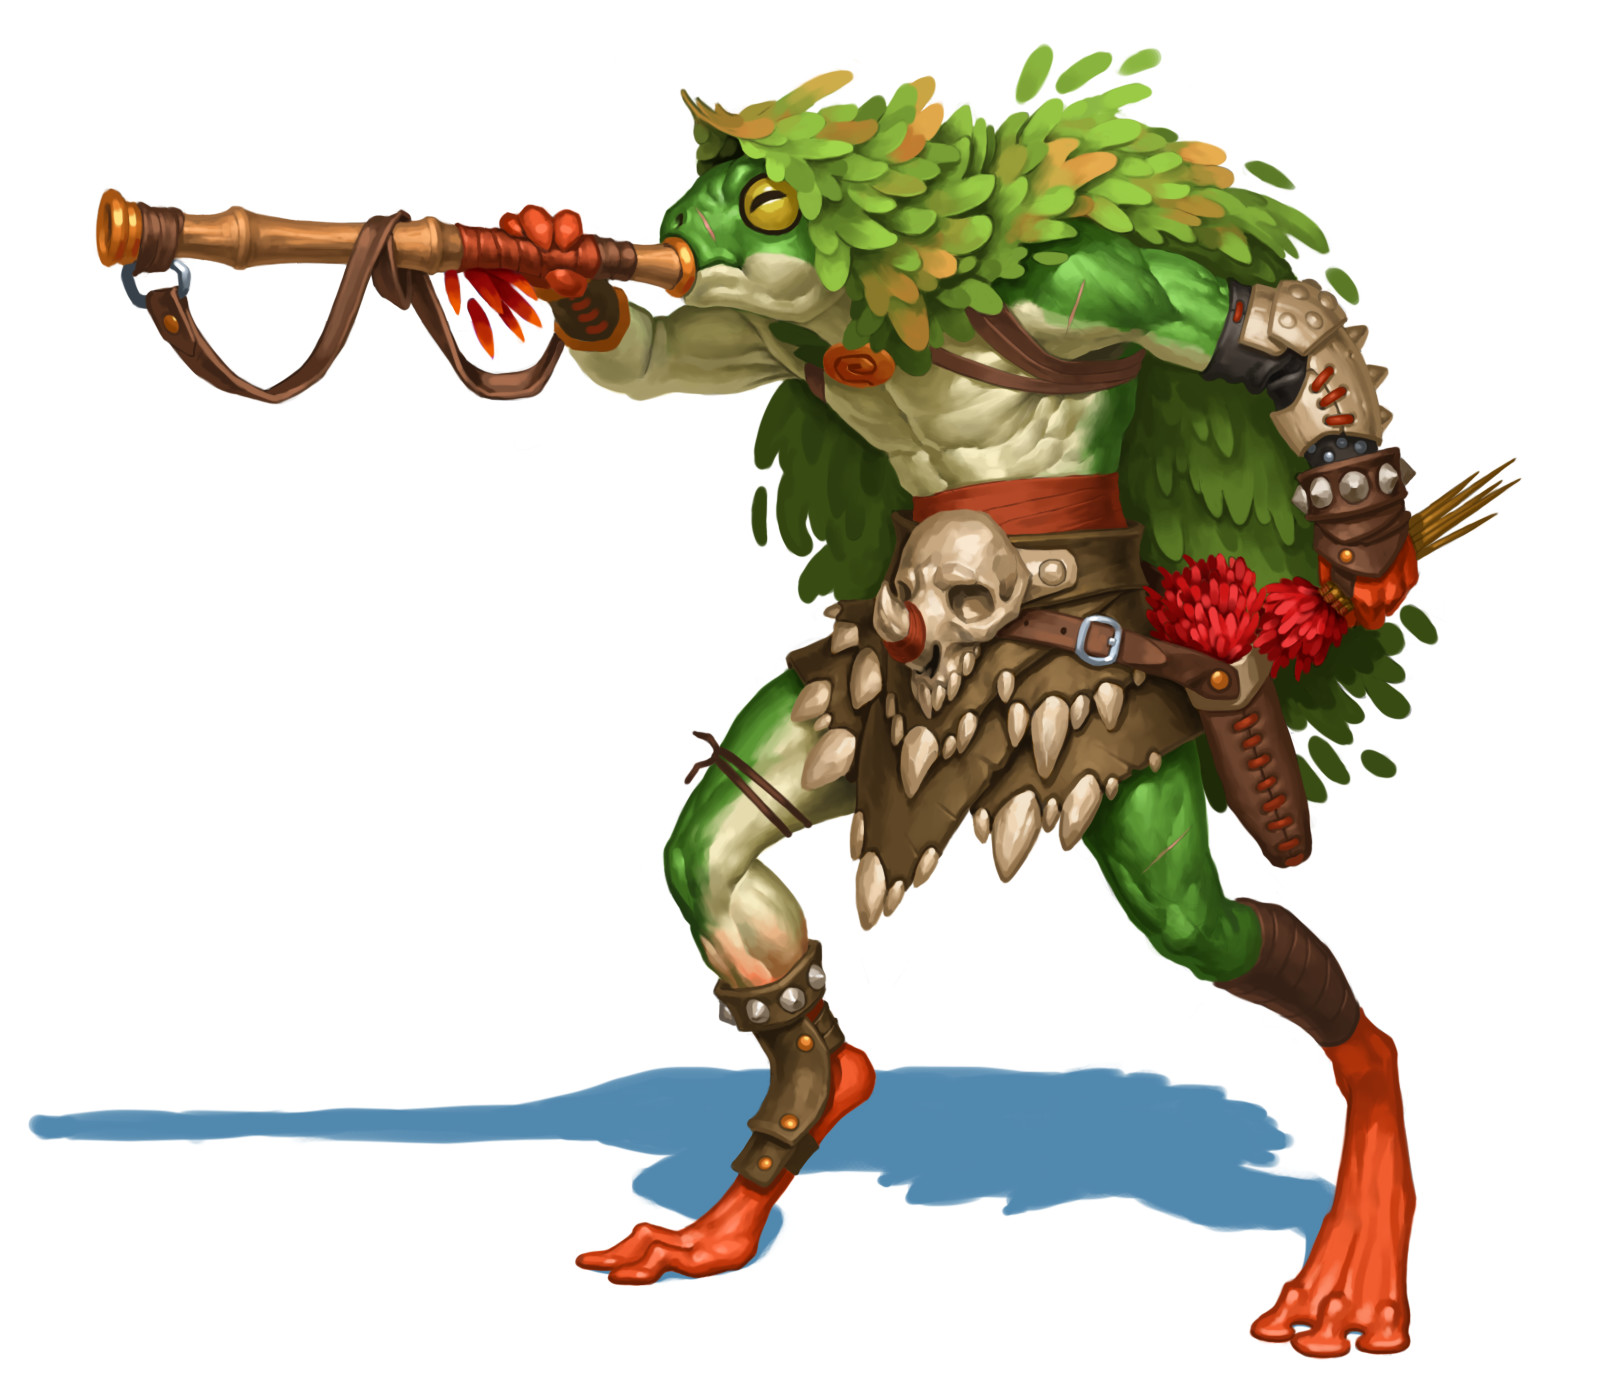
\includegraphics[width=0.48\textwidth]{03kins/img/grung_blowgun.jpg}
\end{figure}

\subsection*{Traits}
Your grung character has an assortment of inborn abilities, part and parcel of grung nature:
\subparagraph{Ability Score Increase} Your Dexterity score increases by 2, and your Constitution score increases by 1.
\subparagraph{Age} Grung reach adulthood in a single year, and can live for up to 80 years.
\subparagraph{Alignment} % Most grungs are lawful, having been raised in a strict caste system.
% Grung society is in constant search of power, and most individual grung look forward to very rare social advancement.
Grungs are in constant search of power, and move along the silver tide.
\subparagraph{Size} Grungs stand between 75 and 105 cm tall and average about 20 kg.
Your size is small.
\subparagraph{Speed} Your base walking speed is 7.5 meters, and you have a climbing speed of 7.5 meters.
\subparagraph{Arboreal Alertness} You have proficiency in the Perception skill.
\subparagraph{Amphibious} You can breathe both air and water.
\subparagraph{Poison Immunity} You are immune to poison damage and the poisoned condition.
\subparagraph{Poisonous Skin} Any creature that grapples you or otherwise comes into direct contact with your skin must succeed on a Constitution saving throw of DC 10 + your Consitution modifier, and become poisoned for 1 minute on a fail.
A poisoned creature no longer in direct contact with you can repeat the saving throw at the end of each of its turns, ending the effect on a success.

You can also apply this poison to any piercing weapon as part of an attack with that weapon. % though when you hit the poison reacts differently.
The target must succeed on the same saving throw or take 2d4 poison damage.
A grung succeeds on these saving throws automatically.

A creature poisoned by a grung suffers an additional effect that varies depending on the grung's skin color.
This effect lasts for one turn and can only be used once per short rest.

\paragraph{Green Toxins} The poisoned creature can't move except to climb or make standing jumps.
If the creature is flying, it can't take any actions or reactions unless it lands.
\paragraph{Blue Toxins} The poisoned creature must shout loudly or otherwise make a loud noise at the start and end of its turns.
\paragraph{Purple Toxins} The poisoned creature feels a desperate need to soak itself in liquid or mud.
It can't take actions or move except to do so or to reach a body of liquid or mud, unless no such body can be found in a 90 meter radius.
\paragraph{Red Toxins} The poisoned creature feels extreme hunger and must use its action to eat something or to move towards a source of food, unless no source of food can be found in a 90 meter radius.
\paragraph{Orange Toxins} The poisoned creature becomes frightened of its allies.
\paragraph{Gold Toxins} The poisoned creature is charmed and permanently learns how to speak basic krehlo.

\subparagraph{Standing Leap} Your long jump is up to 7.5 meters and your high jump is up to 4.5 meters, with or without a running start.
\subparagraph{Grung Weapon Training} Due to combat training, you are proficient with spears, blowguns, and nets.
\subparagraph{Inflatable Cheek Pouches} Due to your frog-like anatomy, you are able to shoot darts at incredible speed.
You can shoot darts with a blowgun to a range of 15/30 meters, and the weapon's damage die is increased to 1d4.
\subparagraph{Water Dependency} If you fail to immerse yourself in water for at least 1 hour during a day, you suffer one level of exhaustion at the end of that day.
You can only recover from this exhaustion by immersing yourself in water for at least 1 hour.
\subparagraph{Languages} You can speak the krehlo tongue and one additional language of your choice, but cannot write or read either.

\begin{figure}[!b]
    \centering
    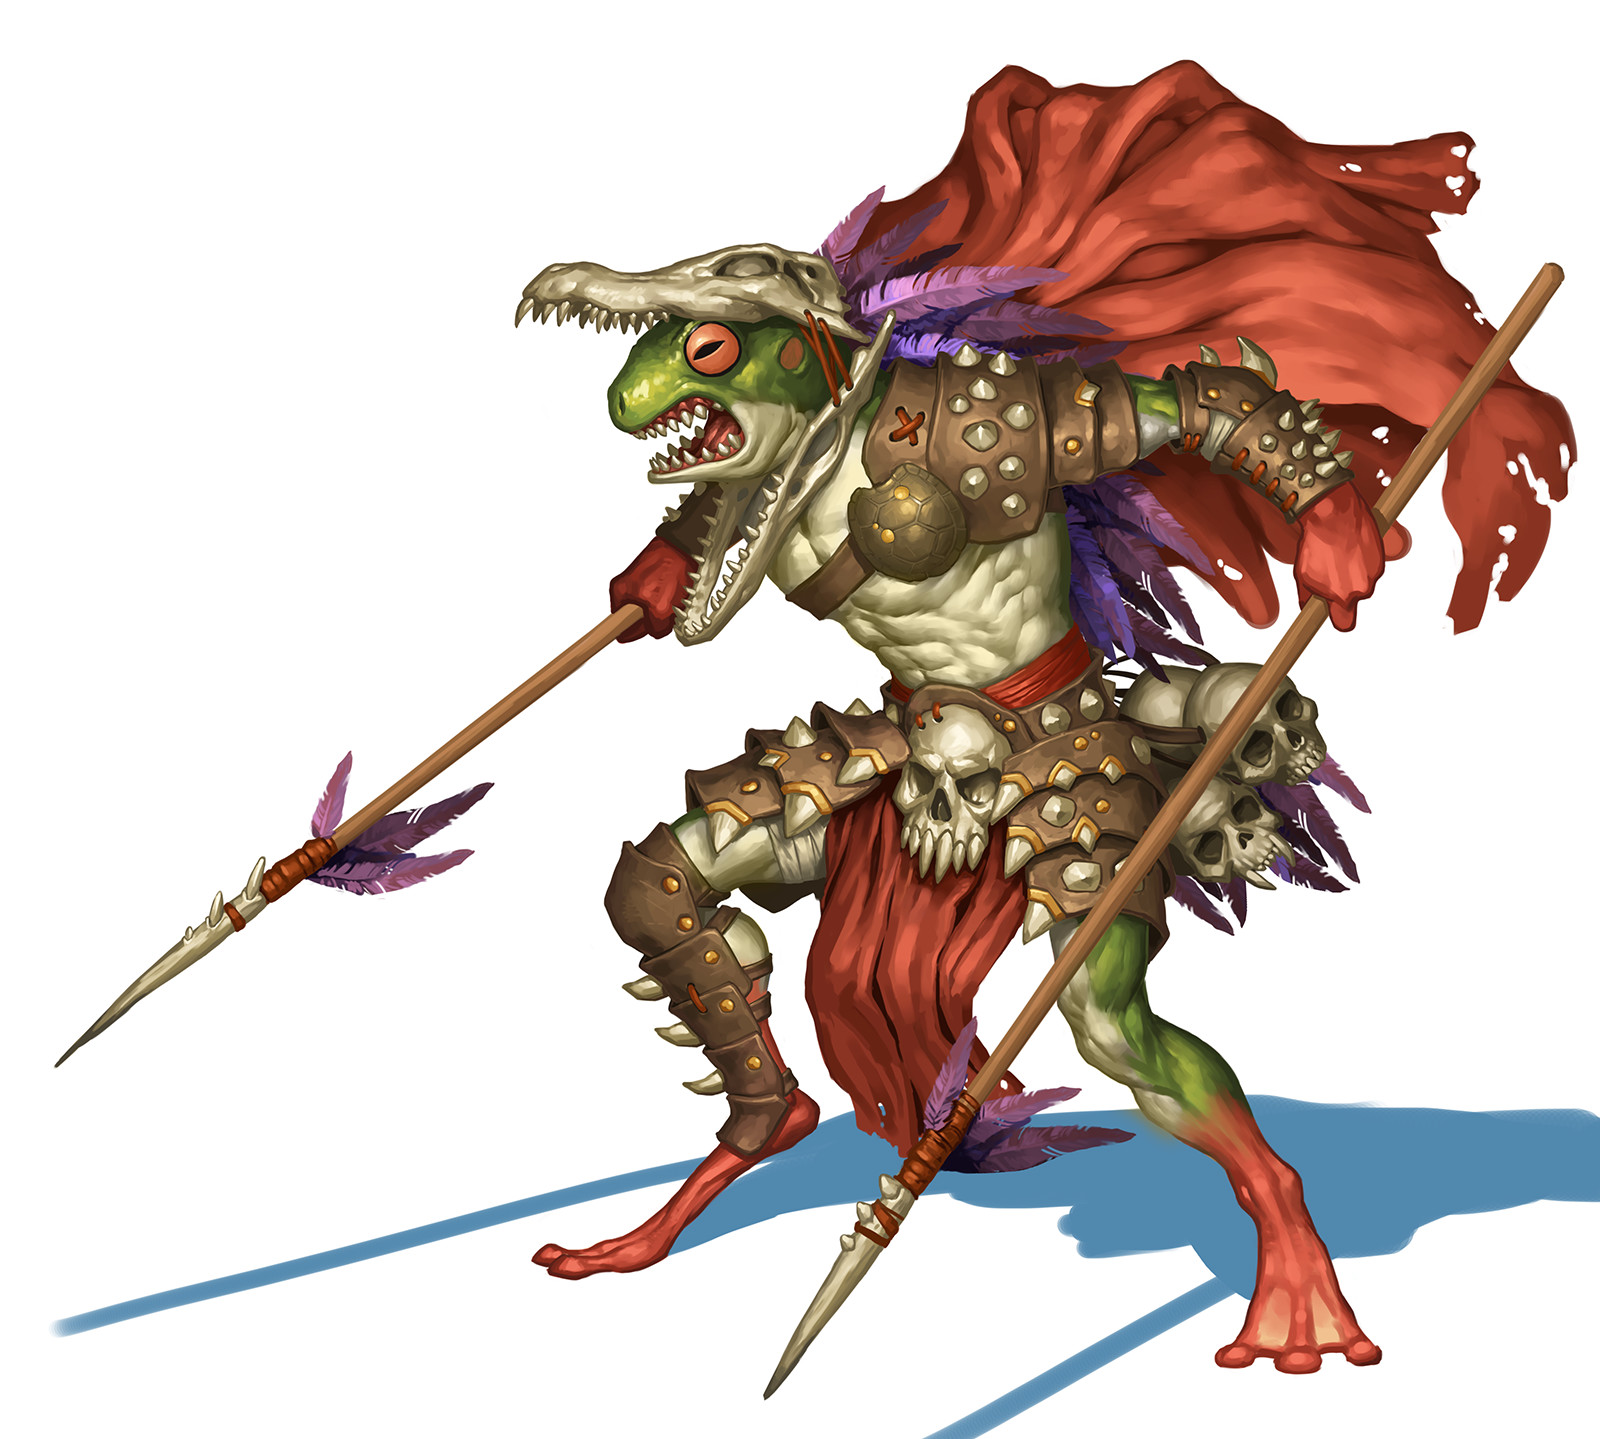
\includegraphics[width=0.48\textwidth]{03kins/img/grung_warrior.jpg}
\end{figure}
\end{linenumbers}
